\section{Validation}

CLAS12 Trigger System Validation was initially performed on data samples simulated by GEANT when system was in design stage. When system was installed cosmic data were used. Finally when beam operation started, validation was compelte and part of entire CLAS12 detector commissioning. Details discussed below.

\subsection{Validation during design phase}

sergey
Validation process consists of several methods and depends on the nature of validated trigger component. For stage1 components written on C++ for HLS/VIVADO implementation,
GEANT-simulated data were processed directly by c++ code and compared with initial similation parameters. 
In addition, the same samples were processed by offline reconstruction software and results compared with the trigger output. 
That double check method practicaly guarantees bug-free implementation. It was no single case when c++ implementation passed validation on
simulated data and failed on final validation stage. Most complicated stage1 components were validated using this method.

ben
Some stage1, as well as all stage2 and stage3 components were implemented using VHDL. For those, VIVADO tools were used for validation diring design phase, in particular ...

\section{Validation of the installed system using cosmic runs} Cole

%\section{Validation on beam during CLAS12 detector commissioning - no FT} Rafo\\

\section{Validation of stage1 triggers using simulations}
Almost all of stage one trigger components, before deploying to the production firmware, were tested on GEANT4 simulated data.

\section{Validation of electron trigger based on ``Beam ON" data}
The ultimate validation of the trigger is done using the so called ''Random Trigger" (RT) runs.
RT runs are special runs, where event readout is initiated not by the trigger logic, but by an external random generator, that
can be tuned on the desired frequency. Most of events in RT runs will not contain any tracks, or other useful information, however,
small fraction of events will have real reconstructed particles which were reconstructed because accidentally detector's response
signal to the particle felled in the readout window that was initiated by the random generator.
Int the event readout in addition to various detector signals, the trigger decisions are stored as well (see section {\color{Red} XX, somewhere above
it should be described, how trigger decisions are made, and what is the clock cycle for trig decisions }).

We want to use these accidental ``Good" events, and check whether corresponding trigger bit is set by trigger logic ({\color{Red} I assume
trigger bits will be described above}).
%%%%%%%%%%%%%%%%%%%%%%%%%%%%%%%%%%%%%%%%% F I G U R E %%%%%%%%%%%%%%%%%%%%%%%%%%%%%%%%%%%%%%%%%%
\begin{figure}[!htb]
 \centering
 \subfloat[]{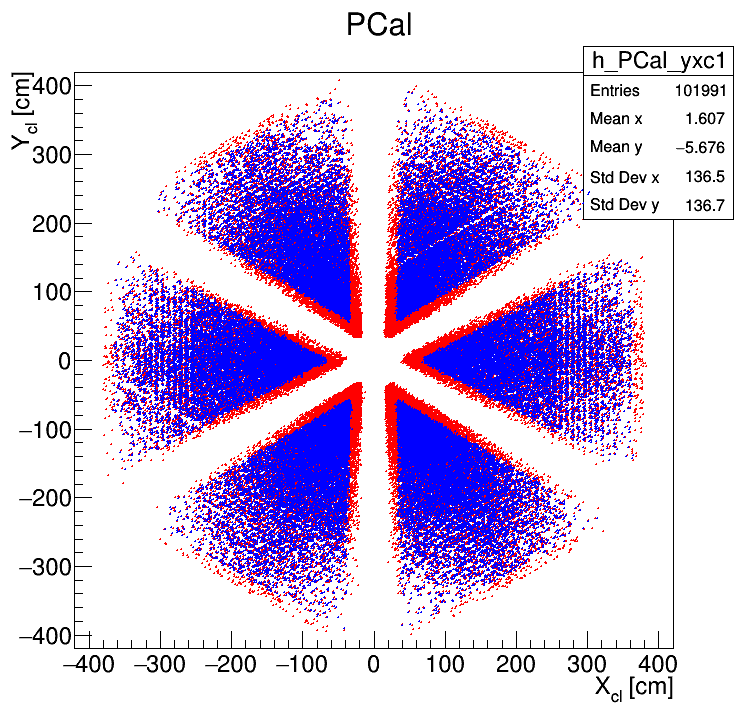
\includegraphics[width=0.24\textwidth]{img/PCal_Fiducials_4878.png}}
 \subfloat[]{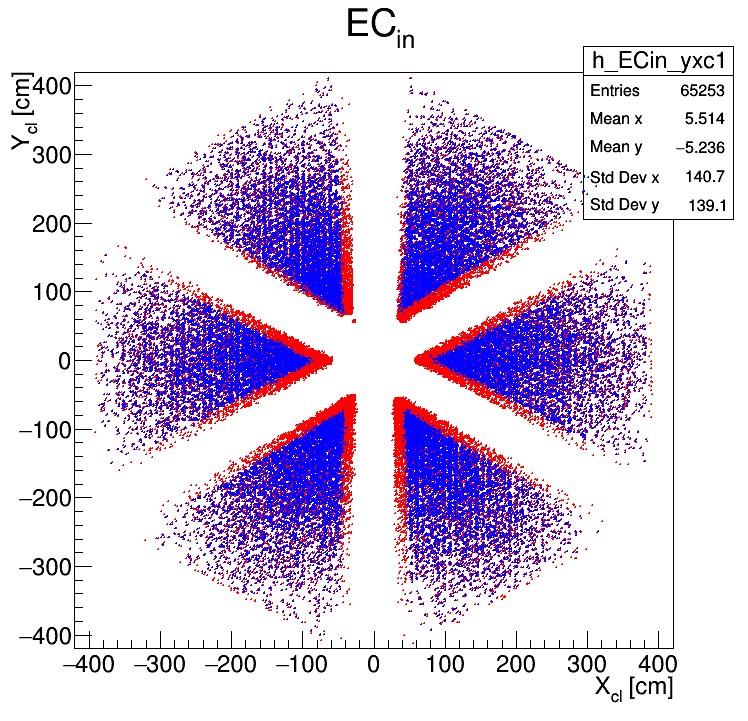
\includegraphics[width=0.24\textwidth]{img/ECin_Fiducials_4878.png}}
 \caption{Distribution of cluster coordinates of PCal (left) and EC\_{in} (right).
 scatter plot in Red shows all events, while blue scatter plot show events where cluster
 is in the fiducial region of the calorimeter (about 15 cm away from the edges).}
\end{figure}
%%%%%%%%%%%%%%%%%%%%%%%%%%%%%%%%%%%%%%%%% F I G U R E %%%%%%%%%%%%%%%%%%%%%%%%%%%%%%%%%%%%%%%%%%

The technique of the trigger validation is the following,
Analysing RT runs, we select 



\section{Validation on beam during CLAS12 detector commissioning - FT} Andrea

.. running c++ code, using VTP banks ..

.. random trigger runs .. 

.. gain calibration check .. 


\section{Validation for different experiments} Valery

After CLAS12 detector was commissioned and trigger system was validated, we still have to repeat validation process occasionally. It is needed because different experiments requesting configuration changes in trigger system, taking advantage of it's flexibility.